%! TEX root = ../thesis.tex
\section{Methodology}%
\label{sec:methodology}

% We first give an introduction to generalized linear models.
% Then, we define the problem and describe our algorithm in detail.
% We also give a probabilistic interpretation and state the limitations of our approach.

\subsection{Generalized Linear Models}%
Generalized linear models (GLMs) are probabilistic models whose likelihood belongs to the exponential family.
Let~$\vx \in \mathbf{R}^D$ be some~$D$-dimensional features, $\vw \in \mathbf{R}^D$ be some~$D$-dimensional parameters, and~$y \in \calD$ be an observation in a given domain~$\calD$.
Let~$h(y) \in \mathbf{R}$ be a scaling factor, $\theta \define \vx\T \vw \in \mathbf{R}$ be the natural parameter, and~$A(\theta) \in \mathbf{R}$ be the log-partition function.
Then, the likelihood of a GLM is
\begin{equation}
	\label{eq:glm}
	p(y \given \vw, \vx) = h(y) \exp{\crl{y \theta - A \rnd{\theta}}}.
\end{equation}

Point-wise predictions are obtained from the mean parameter
\begin{equation*}
	\mu = \E[y] = A'(\theta) = g^{-1}(\theta),
\end{equation*}
where the invertible function~$g : \calD \rightarrow \mathbf{R}$ is called the link function.
This function links the natural parameter and the mean parameter.
The choice of link function depends on the choice of distribution in the GLM.
Equation~\eqref{eq:glm} can be easily generalized to~$K$ outputs~$\vy \in \calD$ (\textit{e.g.}, for multi-party elections) by setting the domain~$\calD$ to be~$K$-dimensional.
One advantage of GLMs is that they can be efficiently fit to data by using convex optimization methods \cite{boyd2004convex}.
In Table~\ref{tab:glm}, we summarize four popular GLMs and their corresponding link functions, natural parameters, mean parameters, and support of~$g$.
We will use these models in our algorithm to predict referenda and elections, as described in the next sections.
We refer the curious reader to \citet[Chapter~9]{murphy2012machine} for a detailed introduction to GLMs.

\begin{table}
	\caption{
		List of GLMs.
		The softmax function is denoted by~$\calS$.
	}
	\label{tab:glm}
	\begin{tabular}{lllll}
		\toprule
		Distrib.                & Link $g$      & $\theta$                        & $\mu$                      & $\calD$        \\
		\midrule

		$\gauss(\mu, \sigma^2)$ & Identity      & $\theta = \mu$                  & $\mu = \vx\T \vw$          & $\mathbf{R}$   \\
		$\gauss(\vmu, \vSigma)$ & Identity      & $\vtheta = \vmu$                & $\vmu = \vX \vw$           & $\mathbf{R}^K$ \\
		$\ber(\mu)$             & Logit         & $\theta = \logit(\mu)$          & $\mu = \sigma(\vx\T \vw)$  & $[0, 1]$       \\
		$\cat(\vmu, K)$         & Inv.\ softmax & $\vtheta = \Softmax^{-1}(\vmu)$ & $\vmu = \Softmax(\vX \vw)$ & $[0, 1]^K$     \\

		\bottomrule
	\end{tabular}
\end{table}

\subsection{Problem Setup}

Let~$\vY \in \real^{R \times (V+1)}$ be the matrix of~$(V+1)$ regional vote results in~$R$ regions, where a result is typically a fraction of votes.
We assume the columns to be in chronological order.
For a new, unobserved vote~$V+1$, we sequentially observe entries of the last column\footnote{This problem can be trivially generalized to multiple unobserved columns~$\{\vy_{V+1}, \vy_{V+2}, \cdots \}$.} in~$\vY$, which we denote by~$\vy_{V+1}$.
Let~$\vY_V \in \mathbf{R}^{R \times V}$ be the \emph{sub-matrix} of all observed, historical results up to vote~$V$.
Denoting the set of consecutive integers by $[R] \coloneq \{1, 2, \ldots, R \}$, we define the set of \textit{observed} indices for the new vote as
\begin{equation*}
	\Obs = \{ r : r \in [R] \text{ and } y_{r,V+1} \in \real \},
\end{equation*}
and the set of \textit{unobserved} indices (corresponding to values to be predicted) as
\begin{equation*}
	\Ubs = \{ r : r \in [R] \text{ and } y_{r,V+1} \equiv \emptyset \}.
\end{equation*}
Let~$\vy^{(\Obs)}_{V+1}$ and~$\vy^{(\Ubs)}_{V+1}$ denote the observed and unobserved entries of~$\vy_{V+1}$, respectively.
Our task is to predict the missing entries~$\vy^{(\Ubs)}_{V+1}$ from~$\vY_V$ and~$\vy^{(\Obs)}_{V+1}$ only.
Figure~\ref{fig:structure} depicts the structure of the matrix~$\vY$.

\begin{figure}
	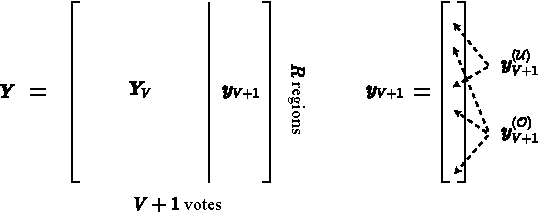
\includegraphics{pdk-structure.pdf}
	\caption{
		Decomposition of the vote matrix~$\vY$ into the fully observed \emph{sub-matrix}~$\vY_V$ and the new vote~$\vy_{V+1}$, whose results arrive sequentially.
		The~$(V+1)$ votes are chronologically ordered and the~$R$ regions are arbitrarily ordered.
	}
	\label{fig:structure}
\end{figure}

To predict the missing entries of~$\vy^{(\Ubs)}_{V+1}$, \citet{etter2016online} use standard matrix factorization with alternating least-squares (ALS) to minimize the non-convex loss based on the Frobenius norm
\begin{equation}
	\label{eq:matrix_factorization}
	\min_{\vA, \vB} \left\Vert \vY^{(\Obs)} - \rnd{\vA\vB^T}^{(\Obs)} \right\Vert_F,
\end{equation}
where~$\vA \in \real^{R \times D}$ and~$\vB \in \real^{V \times D}$ are two matrices of latent dimension~$D \in \mathbf{N}_{>0}$, and where superscript~$(\Obs)$ denotes that, in this case, only the observed entries are kept.
With ALS, each iteration is expensive, and there are neither convergence guarantees nor explicit convergence rates~\cite{bell2007scalable, koren2009matrix}.
According to the Eckart-Young-Mirsky Theorem~\citep{eckart1936approximation}, the optimal solution to Equation~\eqref{eq:matrix_factorization} is the SVD, which is only computable if~$\vY^{(\Obs)}=\vY$.
We devise a more effective algorithm motivated by the special structure of this collaborative filtering problem\cite{etter2016online}.

\subsection{Algorithm}

Our algorithm works in four steps:
First, the fully-observed sub-matrix~$\vY_V$ is decomposed using SVD as
\begin{equation}
	\label{eq:svd}
	\vY_V \approx \vU \vSigma \vV\T,
\end{equation}
where the diagonal matrix~$\vSigma \in \mathbf{R}^{D \times D}$ stores the singular values, and where the matrices~$\vU \in \mathbf{R}^{R \times D}$ and~$\vV \in \mathbf{R}^{V \times D}$ store the~$D$ left and right singular vectors with the highest singular values, respectively.

Second, we compute the projection of the regions into the vote space as
\begin{equation}
	\label{eq:projection}
	\vX = \vY_V \vV = \vU \vSigma,
\end{equation}
where the matrix~$\vX \in \mathbf{R}^{R \times D}$ stores~$D$-dimensional representations of the regions.
We explore these representations in more detail in Section~\ref{sec:experiments}.
These two steps are performed offline, \textit{i.e.}, they are performed once.

Third, we use the observed results of a new vote~$\vy_{V+1}$ and the representations of observed regions in~$\vX$ to fit a GLM~$p$.
We find the maximum likelihood estimate~$\vw_* \in \mathbf{R}^D$ by minimizing the regularized negative log-likelihood of model~$p$ in Equation~\eqref{eq:glm}, with regularization parameter $\lambda \in \mathbf{R}$,
\begin{equation}
	\label{eq:log_likelihood}
	\ell_p(\vw ; \vX, \vy_{V+1}) = -\sum_{r \in \Obs} \log p(y_{r,V+1} \given \vw, \vx_r) + \lambda \| \vw \|_2^2,
\end{equation}
where $y_{r,V+1} \in \mathbf{R}$ is the result of the~$r$-th (observed) region, and~$\vx_r \in \mathbf{R}^D$ is the~$r$-th row of the representation matrix~$\vX$ corresponding to the representation of the~$r$-th region.

Finally, we predict the unobserved regions of the new vote~$\vy_{V+1}^{(\Ubs)} \in \mathbf{R}^{\vert \Ubs \vert}$ as the mean of the GLM~$p$ using the link function~$g$.
From the optimal parameters~$\vw_*$, we compute
\begin{equation}
	\label{eq:prediction}
	\vy^{(\Ubs)}_{V+1} := g^{-1}\left(\vX^{(\Ubs)} \vw_*\right),
\end{equation}
where~$\vX^{(\Ubs)} \in \mathbf{R}^{\vert \Ubs \vert \times D}$ are the representations of the unobserved regions.
The prediction for the national outcome is then the average of $\vy_{V+1}^{(\Obs)}$ and $\vy_{V+1}^{(\Ubs)}$, weighted by the population of each region $r$.
We summarize these steps in Algorithm~\ref{alg:algorithm}.

\begin{algorithm}
	\caption{\textsc{SubSVD-GLM}}
	\label{alg:algorithm}
	\begin{algorithmic}[1]
		\Input Sub-matrix~$\vY_V$, partial results~$\vy_{V+1}$, and GLM~$p$.
		\Output Prediction of unobserved results~$\vy_{V+1}^{(\Ubs)}$.

		\State Decompose $\vY_V \approx \vU \vSigma \vV\T$. \Comment{Equation~\eqref{eq:svd}}
		\State Project $\vX = \vU \vSigma$. \Comment{Equation~\eqref{eq:projection}}
		\State Optimize $\vw_* = \argmin_{\vw} -\ell_p(\vw ; \vX, \vy_{V+1})$. \Comment{Equation~\eqref{eq:log_likelihood}}
		\State Predict $\vy^{(\Ubs)}_{V+1} = g^{-1}\left(\vX^{(\Ubs)} \vw_*\right)$. \Comment{Equation~\eqref{eq:prediction}}

	\end{algorithmic}
\end{algorithm}

To predict the outcomes of referenda and elections, we use the GLMs described in Table~\ref{tab:glm}.
For referenda, we use univariate Gaussian and Bernoulli likelihoods.
For elections, we use multivariate Gaussian and categorical likelihood.
When a univariate Gaussian likelihood is used, the optimal parameters~$\vw_*$ can be learned (step 3 of Algorithm~\ref{alg:algorithm}) in closed form with least-squares
\begin{equation}
	\label{eq:least_squares}
	\vw_* = \rnd{\vX^{(\Obs)\intercal} \vX^{(\Obs)} + \lambda \vI_D }^{-1}\vX^{(\Obs)\intercal} \vy^{(\Obs)}_{V+1},
\end{equation}
where~$\vX^{(\Obs)} \in \mathbf{R}^{\vert \Obs \vert \times D}$ are the representations of the observed regions,~$\vy^{(\Obs)}_{V+1} \in \mathbf{R}^{\vert \Obs \vert}$ are the observed entries of the new vote, and~$\vI_D$ is a~$D$-dimensional identity matrix.
In general, we make the algorithm more efficient by reusing the optimal parameters~$\vw_*$ learned with~$\vert \Obs \vert$ observations when new observations arrive.

Although this algorithm is intuitive, considering the particular structure shown in Figure~\ref{fig:structure}, its general performance is not obvious.
In standard matrix factorization, defined in Equation~\eqref{eq:matrix_factorization}, both~$\vA$ and~$\vB$ are learned together.
Our algorithm fixes~$\vA$ to be equal to~$\vX = \vU \vSigma$, at the expense of adding some constraints, but with the benefit of computational complexity and identifiability gains.
In terms of identifiability, our regularized negative log-likelihood is strictly convex, which now guarantees a unique global optimum.
To limit computational cost, we factorize the matrix~$\vY_V$ only once and reuse its decomposition for each new observation(s) in~$\vy_{V+1}$.
Computing one SVD has complexity~$O(RD^2)$, as typically~$D \leq R$.
The optimization procedure (step 3) can be performed efficiently, \textit{e.g.}, in~$ O(n (\vert \Obs \vert D + D^3))$ for~$n$ iterations of Newton's method.
With a univariate Gaussian likelihood, computing the least-squares solution has asymptotic complexity~$O(\vert \Obs \vert D^2 + D^3)$, which is dominated by the~$\vert \Obs \vert D^2$ term, as typically~$D < \vert \Obs \vert$.
Finally, predicting unobserved values is only a (function of a) matrix-vector multiplication of complexity~$O(\vert \Ubs \vert D)$.

Elections are more complex than referenda because they have categorical outcomes.
Let~$K$ be the number of possible outcomes (for example~$K$ political parties).
The vote result matrix becomes a tensor~$\vY_V \in \real^{R \times V \times K}$.
To apply our algorithm, we concatenate the results of each party to collapse the last dimension.
This yields a matrix~$\vY_V \in \real^{R \times VK}$ that can be decomposed using SVD to obtain representations of regions (steps 1 and 2).
For an election, the regional results are stored in a matrix \mbox{$\vy_{V+1} \in \mathbf{R}^{R \times K}$}, and we use multivariate Gaussian or categorical likelihoods in the GLM to model the multiple outcomes (steps 3 and 4).

% TODO: Add sentences about how to obtain final prediction by aggregating observed results and predicted results.
% TODO: Mention that categorical distribution is equivalent to the multinomial distribution with N=1 (one trial).
% TODO: Define the softmax function in a footnote.
% TODO: Mention that we can include a bias term in the weights to learn the offset.

\subsection{Probabilistic Interpretation}

Voting data have the special property that the sum of all possible outcomes in a given region is equal to 1.
The outcome~$p \in [0, 1]$ of a referendum is the probability~$p$ that it is accepted (and the probability~$1-p$ that it is rejected).
The suffrage~$\vp \in [0, 1]^K$ obtained by~$K$ political parties in an election describes the probability mass function~$p(k)$ that the~$k$-th party is elected.
As a result, we provide a probabilistic interpretation of outcomes of referenda and elections.

Let~$P_{rv}^{(i)} \sim \bernoulli(p_{rv})$ be a random variable representing the vote cast by voter~$i$ in region~$r$ on referendum~$v$.
As voting is anonymous, we do not observe individual votes, rather the average vote in each region
\begin{equation*}
	\frac{1}{N_r} \sum_{i=1}^{N_r} P_{rv}^{(i)},
\end{equation*}
where~$N_r$ is the number of voters in region~$r$, and whose expectation is $p_{rv}$.
By decomposing the result matrix~$\vY = \vA \vB\T$ as in Equation~\eqref{eq:matrix_factorization}, we posit that the parameter of the random variables describing individual voters is a product of latent features of regions and votes~$p_{rv} = \va_r\T \vb_v$, with~$\va_r, \vb_v \in \mathbf{R}^D$.
In Equation~\eqref{eq:svd} and Equation~\eqref{eq:projection}, our algorithm learns the latent features of the regions~$\va_r = \rnd{\vU \vSigma}_r = \vx_r$ from historical data.
In Equation~\eqref{eq:log_likelihood}, it learns the latent features of the votes~$\vb_v = \argmin_{\vb} -\ell_p(\vb ; \vX, \vy_v)$ as the parameters of a GLM~$p$.

So far, we have considered that each region has the same number of voters.
If we have access to data about the number of voters in each region (\textit{e.g.}, the number of valid votes, the number of eligible voters, or the population), we can include this information by replacing the regularized log-likelihood in \eqref{eq:log_likelihood} by
\begin{equation}
	\label{eq:weighted}
	-\ell_p(\vw ; \vX, \vy_{V+1}) = \sum_{r \in \Obs} N_r \log p(y_{r,V+1} \given \vw, \vx_r) + \lambda \Vert \vw \Vert_2^2,
\end{equation}
where $N_r \in \mathbf{R}$ is a count related to the number of voters in region~$r$.
We refer to the variation of the algorithm that uses this log-likelihood as \textit{weighted}.
We refer to the variation of the algorithm that uses the log-likelihood in \eqref{eq:log_likelihood} as \textit{unweighted}.
A similar argument can be trivially made for elections by letting~$P_{rv}^{(i)} \sim \categorical(p_{rv}, K)$ be a random variable describing the vote cast by voter~$i$ in region~$r$ on vote~$v$ for $K$ political parties.

\subsection{Limitations}

By design, our approach suffers from the cold-start problem of collaborative filtering~\cite{koren2009matrix}.
We can make predictions only when at least one past observation is available, \textit{i.e.}, when~$\vert \Obs \vert = 1$.
To bypass this problem, \citet{etter2016online} include features of the regions, such as the geographical location, the population size, and the elevation, and features of the votes, such as the voting recommendation by political parties.
These features are, however, not systematically and programmatically available, making it difficult to use them in a real-world system such as the one we describe in Section~\ref{sec:depsys}.

Our approach also makes the hypothesis that regional and vote representations are static over time.
In particular, the algorithm learns the regional representations over the whole training set.
The latest results might, however, provide more information than older results.
To bypass this problem, we could weigh the SVD by using a sliding window or by exploiting a temporal SVD algorithm \cite{bamler2017dynamic} to capture the dynamics of the voting process.

% Other sources of data, \textit{e.g.}, polling data, could be used to make predictions prior to a vote.
% However, the business model of polling agencies often solely relies on their data, which prevents them from sharing their datasets.
% Textual data, for example extracted from the actual law proposal or from parties documents would also constitute valuable data.
% But the specificity of legal text makes it difficult to process and exploit such datasets, and we keep this direction as future work.
